\section{Experiments}

\begin{figure}[t]
\centering
\begin{tikzpicture}[
    stage/.style={draw, rounded corners, fill=blue!8, minimum width=3.0cm, minimum height=0.9cm, align=center, font=\small},
    hyp/.style={draw, rounded corners, fill=orange!10, minimum width=2.4cm, minimum height=0.6cm, align=center, font=\footnotesize},
    result/.style={draw, rounded corners, fill=green!10, minimum width=2.4cm, minimum height=0.6cm, align=center, font=\footnotesize},
    arr/.style={-{Stealth[length=5pt]}, thick},
    note/.style={font=\scriptsize\itshape, text=gray!70!black},
]

\node[stage] (ode) {Stage 1:\\Delayed Replicator ODE};
\node[stage, right=2.2cm of ode] (sim) {Stage 2:\\Networked Simulation};
\node[stage, right=2.2cm of sim] (class) {Regime\\Classification};

\node[hyp, below=0.7cm of ode] (h1) {H1: Delay destabilizes};
\node[hyp, below=0.15cm of h1] (h2) {H2: Sharpness amplifies};
\node[hyp, below=0.15cm of h2] (h3) {H3: Mixed pop.\ fragile};

\node[result, below=0.7cm of sim] (e0) {Exp.~1: ODE valid.};
\node[result, below=0.15cm of e0] (e1) {Exp.~2: Discrete bridge};
\node[result, below=0.15cm of e1] (e23) {Exp.~3--4: Sweeps};
\node[result, below=0.15cm of e23] (e4) {Exp.~5: Crossed design};
\node[result, below=0.15cm of e4] (e5) {Exp.~6: RL regulator};

\node[result, below=0.7cm of class] (rq1) {Q1: Survives? \checkmark};
\node[result, below=0.15cm of rq1] (rq2) {Q2: Sharpness? \checkmark};
\node[result, below=0.15cm of rq2] (rq3) {Q3: Learning buffers};
\node[result, below=0.15cm of rq3] (rq4) {Q4: RL regulator?};

\draw[arr] (ode) -- node[above, note] {hypotheses} (sim);
\draw[arr] (sim) -- node[above, note] {50 seeds/cond.} (class);

\draw[arr, gray] (ode) -- (h1);
\draw[arr, gray] (sim) -- (e0);
\draw[arr, gray] (class) -- (rq1);

\node[above=0.15cm of ode, note] {Section 2};
\node[above=0.15cm of sim, note] {Sections 3--4};
\node[above=0.15cm of class, note] {Section 4};

\end{tikzpicture}
\caption{Solution pipeline. Stage~1 derives analytical predictions from the delayed replicator ODE. Stage~2 tests these predictions in a networked agent-based simulation with three decision architectures. Regime classification assigns each run to stable, oscillatory, or runaway. The mapping from hypotheses (H1--H3) through experiments (1--6) to research questions (Q1--Q4) is detailed in Table~\ref{tab:experiment_map}.}
\label{fig:pipeline}
\end{figure}

The analytical theory (Section~2) establishes that delay can destabilize a well-mixed population with a fixed strategy-revision rule. The simulation model (Section~3) introduces three layers of realism: finite heterogeneous populations, network structure, and adaptive learning via reinforcement learning. The experiments address the following research questions:

\begin{enumerate}
\item Does the delay-destabilization mechanism survive in the networked simulation? The ODE predicts instability above $\Delta_c$; the simulation adds noise, discretization, and network effects that could either amplify or suppress this mechanism.
\item How does sigmoid sharpness $k$ interact with delay? The theory predicts that higher $k$ lowers $\Delta_c$ (Equation~\ref{eq:deltac_sigmoid}). We test whether the simulation reproduces this monotonic relationship.
\item Does adaptive learning amplify or buffer delay-induced instability? The naive expectation is that learning agents exploit delayed low-alarm windows more effectively, amplifying instability. The alternative is that cumulative learning provides implicit memory that dampens oscillations.
\item Can an adaptive regulator compensate for the destabilizing effect of adaptive agents? If agents learn to exploit delay, can an RL-trained regulator learn to counteract them?
\end{enumerate}

Table~\ref{tab:experiment_map} maps each experiment to the research question it addresses and the key controlled variables.

\begin{table}[ht]
\centering
\begin{tabular}{llll}
\toprule
Experiment & Research question & Varied factor & Controlled factors \\
\midrule
Experiment~1: ODE validation & Baseline & $\Delta/\Delta_c$ & Continuous ODE \\
Experiment~2: Discrete mean-field & Q1 (discretization) & $\eta$, $\Delta$ & Mean-field, no network \\
Experiment~3: Delay sweep & Q1 & $\Delta$ & $k{=}20$, Q-learning \\
Experiment~4: Sharpness sweep & Q2 & $k$ & $\Delta{=}15$, Q-learning \\
Experiment~5: Crossed design & Q3 & $\Delta \times$ architecture & $k{=}10$, 3 architectures \\
Experiment~6: RL regulator & Q4 & Regulator type & $\Delta{=}6$, Q-learning \\
\bottomrule
\end{tabular}
\caption{Mapping of experiments to research questions. Each experiment varies one factor while controlling others to isolate the effect. Experiment~1 and Experiment~2 validate the analytical theory; Experiment~3 through Experiment~6 test the hypotheses in the full simulation.}
\label{tab:experiment_map}
\end{table}

The progression is deliberate: Experiment~1 confirms the ODE theory is mathematically correct; Experiment~2 bridges continuous and discrete dynamics; Experiment~3 and Experiment~4 establish dose-response curves for delay and sharpness; Experiment~5 is the central experiment testing the interaction between delay and agent architecture; Experiment~6 is exploratory. All results reported in this section use 50 independent seeds per condition. Raw time-series histories, summary statistics, and configuration manifests are stored under \texttt{experiments/results/paper1\_v2/} with per-experiment subdirectories. The progression from ODE validation through discrete mean-field to full network simulation reveals both the robustness of the core delay-instability mechanism and the quantitative gaps introduced by agent heterogeneity and adaptive learning.

\subsection{Experimental setup}

\paragraph{Shared settings.} All networked experiments use $N=240$ agents on a modular stochastic block model graph (6 communities of 40 nodes, intra-community edge probability $p_{\mathrm{in}}=0.08$, inter-community $p_{\mathrm{out}}=0.004$). The population size $N{=}240$ is large enough for stable mean-field-like alarm statistics but small enough for complete Q-table exploration within 500 steps. The 6-community modular structure follows standard stochastic block model designs \citep{holland1983stochastic} and produces well-defined bridge nodes for the companion paper's analysis; the intra/inter edge probabilities ($0.08/0.004$) yield a modularity ratio of $p_{\mathrm{in}}/p_{\mathrm{out}}=20$, ensuring clear community separation. The simulation horizon is 500 time steps, sufficient for Q-learning agents to reach stable policies (convergence diagnostic below confirms Q-values equilibrate by step 100--200). We use 50 independent seeds per condition throughout, with results frozen after completion to ensure reproducibility. The sharpness parameter $k$ is set high ($k=10$ or $k=20$) to ensure the system operates above the critical threshold $\Delta_c$ at the tested delay values; lower $k$ would require longer delays to produce measurable effects. The alarm threshold $A_c$ is set to the theoretical equilibrium level. These parameter choices follow from the analytical predictions: we choose settings where the theory predicts instability and test whether the simulation confirms it.

\paragraph{Baselines and comparison strategy.} This paper studies a mechanism (delay-induced instability), not a method that competes against alternatives on a benchmark. The natural baselines are therefore \emph{ablation baselines}: conditions that remove specific components of the mechanism to isolate their contribution. Fixed-policy agents serve as the null model (no feedback loop, so delay cannot destabilize). Reactive agents isolate the effect of memoryless reactivity. Q-learning agents add adaptive memory. The comparison across these three architectures answers Q3. No prior work has studied the specific interaction between institutional delay, agent learning, and network structure that we examine; accordingly, we compare agent architectures rather than competing models from the literature. The ODE validation (Experiment~1) and discrete mean-field (Experiment~2) serve as additional baselines connecting the simulation to the analytical theory.

\paragraph{Regime classification.} Each simulation run is classified into one of three regimes based on tail-half statistics (the final 50\% of the time series, after transient dynamics decay). \emph{Stable}: the radical fraction remains below the runaway threshold $R_{\max}=0.40$ and oscillation amplitude is small. \emph{Oscillatory}: substantial periodic variation in radical fraction (detected by spectral analysis: peak-to-total power ratio $>0.25$ with amplitude $>0.08$, or a fallback test of tail amplitude $>0.12$ or tail standard deviation $>0.04$) without exceeding $R_{\max}$. \emph{Runaway}: the maximum radical fraction exceeds $R_{\max}=0.40$. We emphasize that ``runaway'' denotes crossing this threshold, not unbounded growth: across all runs so labeled, the tail-period mean radical fraction never exceeds $0.30$, consistent with the supercritical-Hopf prediction of bounded limit cycles rather than literal radical domination. The threshold $R_{\max}=0.40$ is chosen as a substantively meaningful level at which radical agents dominate; we verify that the central ordering (fixed $\leq$ Q-learning $\leq$ reactive in delay sensitivity) is preserved across thresholds from 0.30 to 0.50 (Section~5).

\subsection{Theory validation (Experiment~1, Experiment~2)}

\paragraph{Experiment~1: ODE validation.} This experiment validates the analytical theory by numerically integrating the delayed replicator equation~\eqref{eq:delayed_rep} directly, sweeping $\Delta$ from $0$ to $4\Delta_c$. It is the ground-truth baseline: if the ODE does not bifurcate at $\Delta_c$, the theory is wrong and the simulation experiments are moot. The integration uses parameter values $a{=}2.0$, $C{=}7.0$, $k{=}10$, $x_c{=}0.72$, representative magnitudes chosen so that the interior equilibrium $x^*{\approx}0.63$ sits at a non-degenerate point away from the boundaries, with critical delay $\Delta_c{\approx}0.47$. The supercriticality proof (Appendix~\ref{app:hopf_proof}) shows the qualitative bifurcation is insensitive to these specific values across all admissible parameters.

Direct numerical integration of Equation~\eqref{eq:delayed_rep} confirms Theorem~\ref{thm:critical_delay}. Figure~\ref{fig:ode_bifurcation} shows the bifurcation diagram: below $\Delta_c$, trajectories converge to $x^*$; at $\Delta/\Delta_c=1$, stable limit cycles emerge with amplitude growing continuously from zero, consistent with the supercritical Hopf bifurcation. Figure~\ref{fig:ode_delay_sweep} shows representative trajectories, and Figure~\ref{fig:ode_k_sweep} shows that increasing sharpness $k$ at fixed $\Delta/\Delta_c = 1.5$ sharpens the nonlinear response and increases limit-cycle amplitude.

\begin{figure}[ht]
\centering
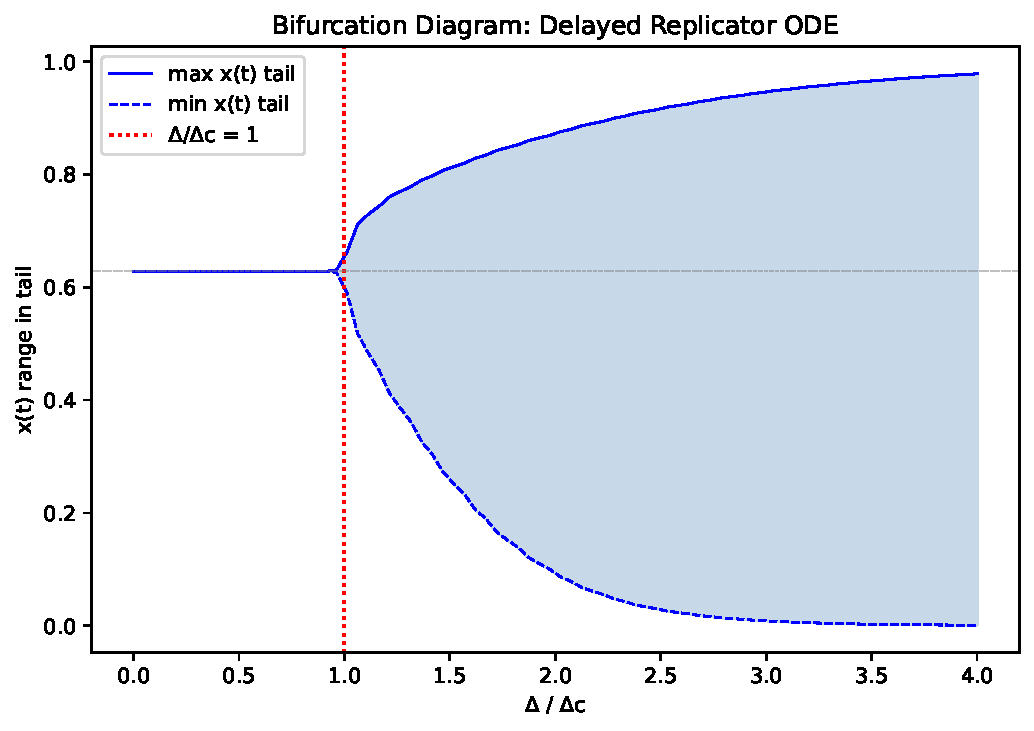
\includegraphics[width=0.85\textwidth]{figures/fig_ode_bifurcation.pdf}
\caption{Bifurcation diagram for the delayed replicator ODE (Experiment~1). Horizontal axis: normalized delay $\Delta/\Delta_c$. Below $\Delta_c$, the equilibrium is stable. At $\Delta/\Delta_c=1$, a Hopf bifurcation produces stable limit cycles with continuously growing amplitude (solid: numerical envelope; dashed: theoretical threshold). \textbf{Conclusion:} the analytical theory (Theorem~\ref{thm:critical_delay}) is confirmed exactly---the instability occurs precisely at the predicted threshold.}
\label{fig:ode_bifurcation}
\end{figure}

\begin{figure}[ht]
\centering
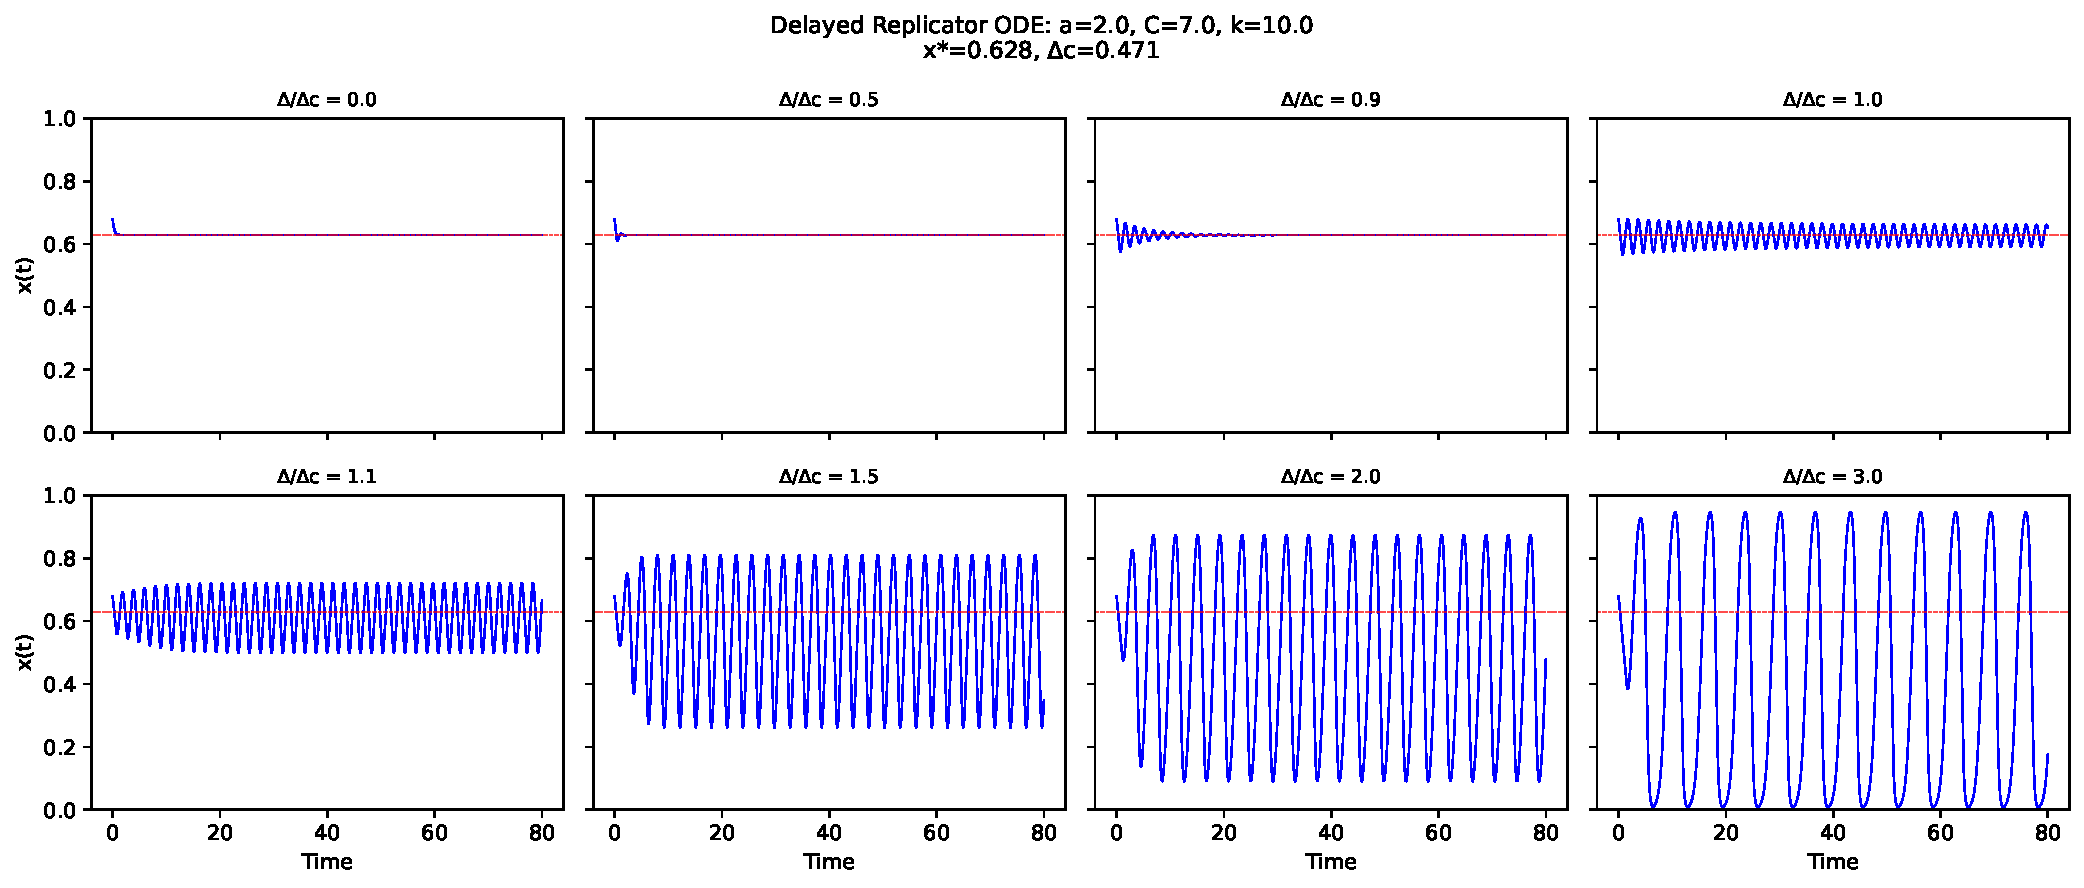
\includegraphics[width=0.85\textwidth]{figures/fig_ode_delay_sweep.pdf}
\caption{Representative ODE trajectories at six delay levels (Experiment~1). Below $\Delta_c$: damped convergence to equilibrium. Above: sustained limit cycles with amplitude growing with $\Delta$. The transition is sharp, consistent with the supercritical Hopf bifurcation (Proposition~\ref{prop:supercritical}).}
\label{fig:ode_delay_sweep}
\end{figure}

\begin{figure}[ht]
\centering
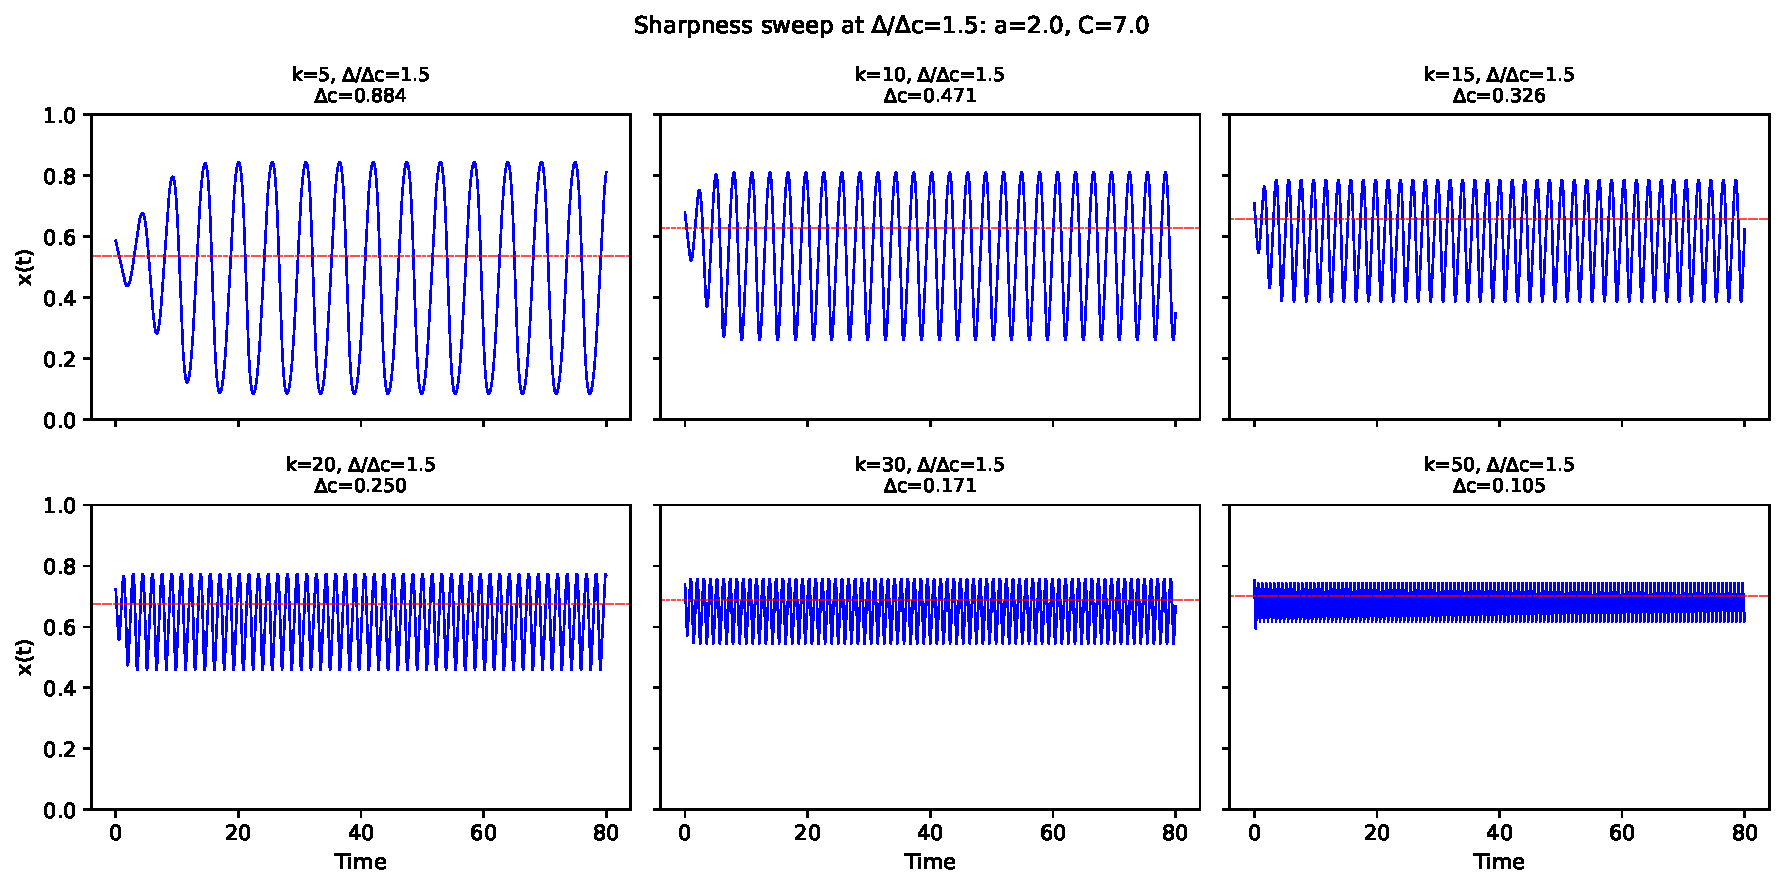
\includegraphics[width=0.85\textwidth]{figures/fig_ode_k_sweep.pdf}
\caption{Effect of sharpness $k$ on ODE dynamics at fixed $\Delta/\Delta_c = 1.5$ (Experiment~1). All panels are at the same distance beyond the stability boundary, yet higher $k$ produces sharper, larger-amplitude limit cycles saturating near the population boundaries. \textbf{Conclusion:} sharpness amplifies the nonlinear consequences of delay-induced instability, confirming Hypothesis~2.}
\label{fig:ode_k_sweep}
\end{figure}

\paragraph{Experiment~2: Discrete mean-field.} This experiment bridges continuous ODE dynamics and discrete multi-agent simulation. Discretization itself can introduce instabilities absent in the continuous limit \citep{alboszta2004stability}. We study a discrete-time mean-field system with step size $\eta$ and verify that the continuous bifurcation structure is recovered as $\eta\to 0$. This isolates discretization effects from network structure, agent heterogeneity, and learning.

Figure~\ref{fig:discrete_mf_phase} presents the phase diagram in $(\Delta, \eta)$ space. For small $\eta$, the discrete system recovers the ODE bifurcation structure. As $\eta$ increases, the stability margin narrows and the dynamics overshoot the ODE limit-cycle amplitude (Figure~\ref{fig:discrete_mf_trajectories}). Figure~\ref{fig:discrete_mf_eta} quantifies this: the stability margin decreases monotonically with $\eta$. This establishes that discretization introduces additional instability beyond delay. The result provides a baseline for interpreting the full simulation, where discrete time steps are inherent.

\begin{figure}[ht]
\centering
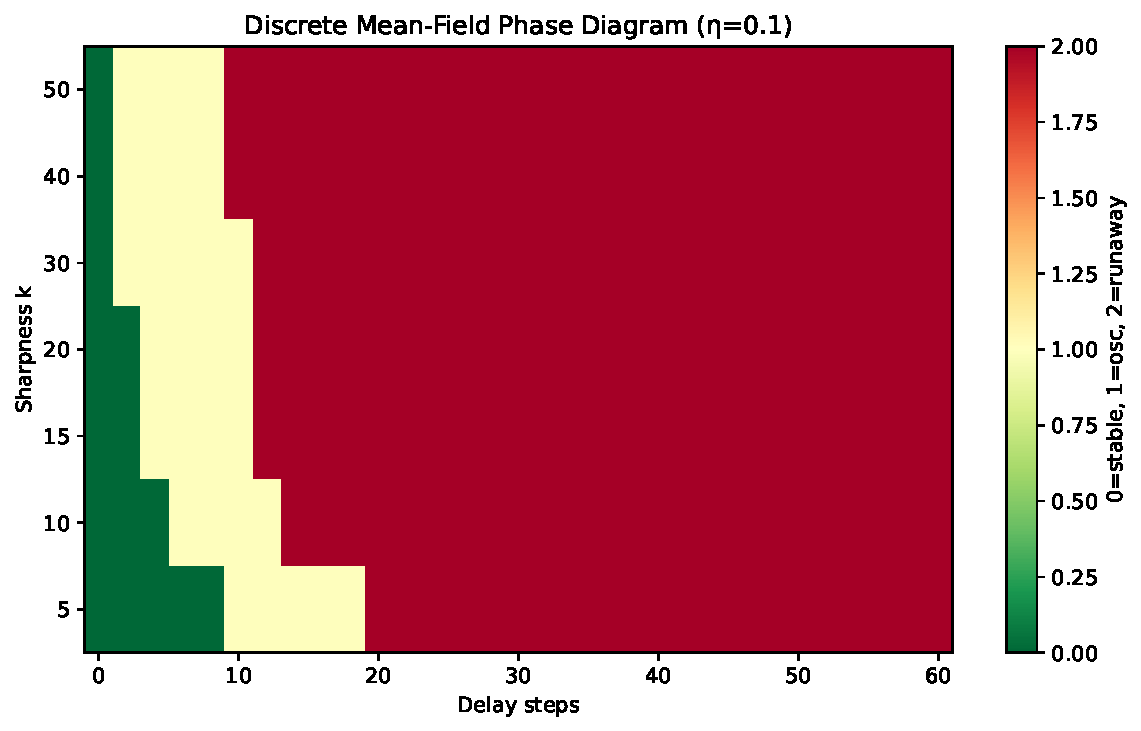
\includegraphics[width=0.75\textwidth]{figures/fig_discrete_mf_phase.pdf}
\caption{Phase diagram of the discrete mean-field system in $(\Delta, \eta)$ space (Experiment~2). Color: regime classification. \textbf{Conclusion:} the stability region contracts with increasing $\eta$, confirming that discretization itself is an additional instability source---the full simulation's discrete time steps make the system \emph{more} fragile than the ODE predicts.}
\label{fig:discrete_mf_phase}
\end{figure}

\begin{figure}[ht]
\centering
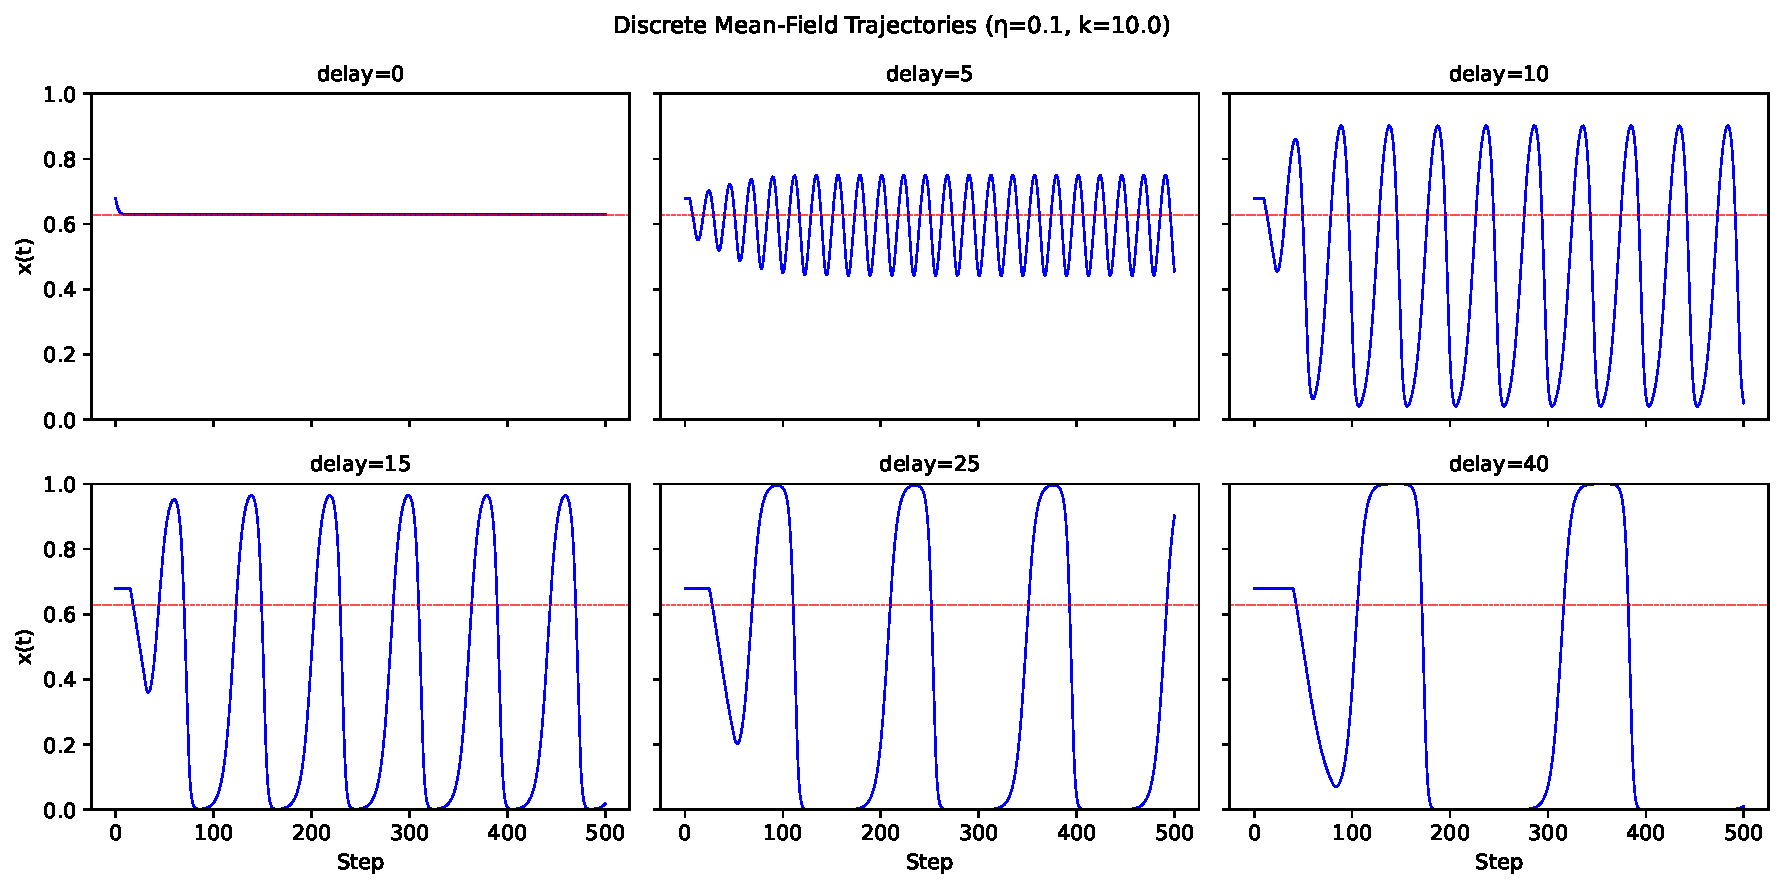
\includegraphics[width=0.85\textwidth]{figures/fig_discrete_mf_trajectories.pdf}
\caption{Discrete mean-field trajectories at $\Delta{=}1.2\Delta_c$ for several $\eta$ values (Experiment~2). Small $\eta$: bounded oscillations matching the ODE limit cycle. Large $\eta$: overshooting dynamics exceeding the ODE envelope. \textbf{Conclusion:} the full simulation's discrete time steps ($\eta \approx 1$) introduce additional instability beyond the continuous theory.}
\label{fig:discrete_mf_trajectories}
\end{figure}

\begin{figure}[ht]
\centering
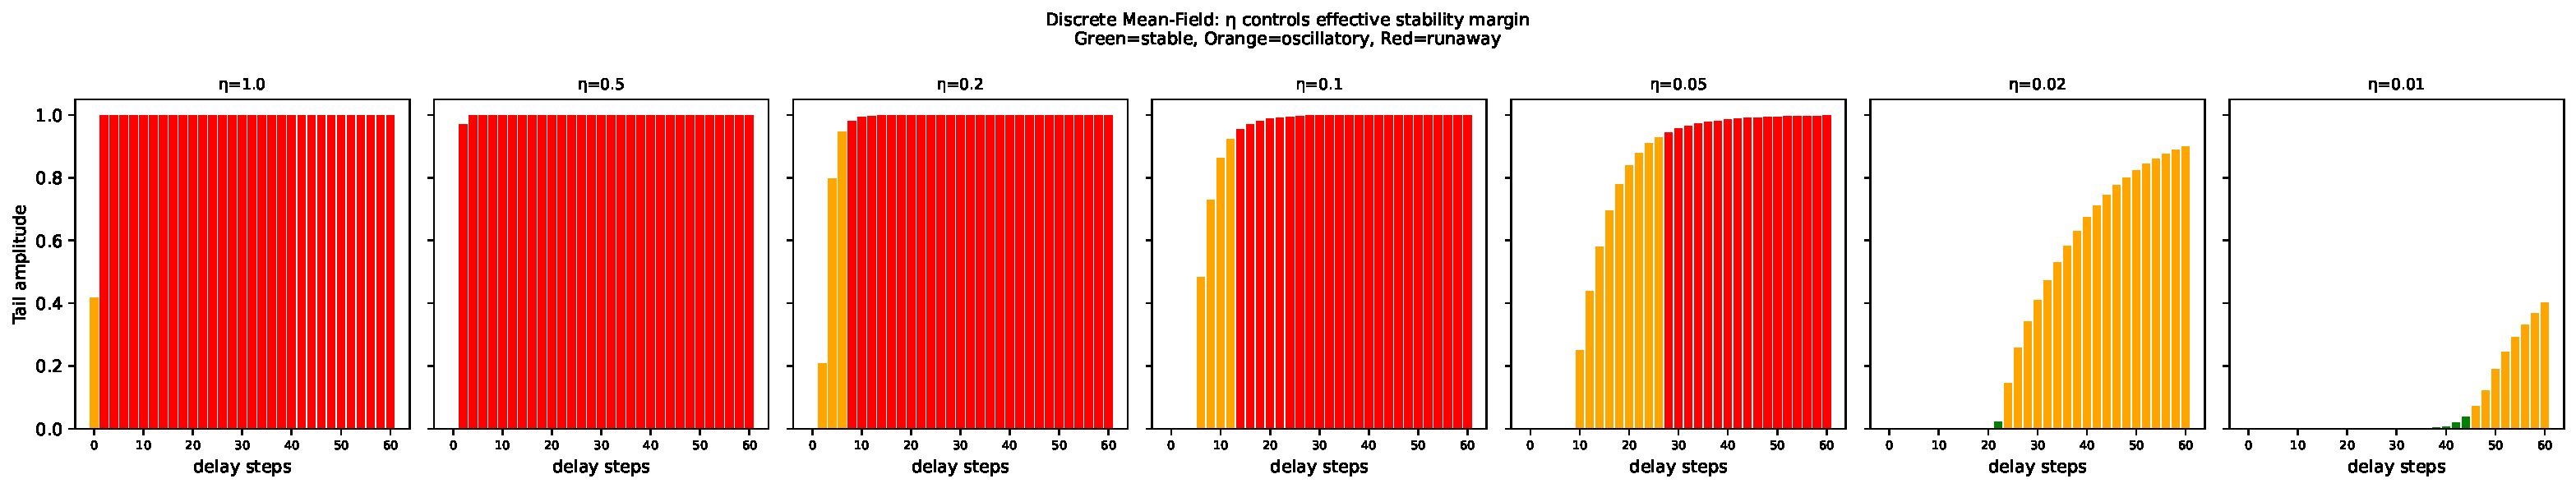
\includegraphics[width=0.6\textwidth]{figures/fig_discrete_mf_eta.pdf}
\caption{Stability margin vs.\ discrete step size $\eta$ (Experiment~2). As $\eta\to 0$, the margin recovers $\Delta_c$ from the continuous theory. \textbf{Conclusion:} discretization reduces the stability margin monotonically. This provides a quantitative bridge between the ODE prediction and the simulation's inherent discrete dynamics.}
\label{fig:discrete_mf_eta}
\end{figure}

\subsection{Dose-response (Experiment~3, Experiment~4)}

\paragraph{Experiment~3: Delay sweep.} This experiment tests Hypothesis~1 (delay destabilizes) in the full networked simulation with Q-learning agents. We sweep repression delay from 0 to 30 steps using $k{=}20$ (placing the system well above $\Delta_c$) and 500 time steps (sufficient for Q-value convergence). If the ODE mechanism survives, runaway frequency should increase monotonically with delay.

Table~\ref{tab:delay_sweep} reports runaway rate vs.\ delay ($k{=}20$, Q-learning agents). At delay${}{=}0$ the system is already only 46\% stable (44\% oscillatory, 10\% runaway): the non-delayed dynamics sit near the oscillatory boundary, and the 10\% runaway reflects stochastic noise rather than delay (Theorem~\ref{thm:nodelay}). Increasing delay shifts this distribution decisively into runaway, which rises to 72\% at delay${}{=}30$ (95\% confidence interval (CI) $[58\%, 83\%]$), an excess of $+62$ percentage points over the delay-zero runaway floor. The monotonic trend confirms the qualitative prediction: delay converts the marginally-stable baseline into large-amplitude runaway. Sixty-two percentage points is not a subtle effect. This sweep uses Q-learning agents, whose adaptive exploration leaves them near the oscillatory boundary even at $\Delta=0$; the cleanest demonstration of destabilization from a \emph{fully} stable baseline is the reactive architecture (Experiment~5 and Figure~\ref{fig:reactive_fine}), which is 100\% stable at $\Delta=0$ and collapses entirely once delay is introduced.

\begin{table}[ht]
\centering
\begin{tabular}{lccc}
\toprule
Delay (steps) & Runaway rate & 95\% CI & Excess over $\Delta{=}0$ (pp) \\
\midrule
0  & 0.10 & $[0.04, 0.21]$ & --- \\
2  & 0.12 & $[0.06, 0.24]$ & $+2$ pp \\
4  & 0.20 & $[0.11, 0.33]$ & $+10$ pp \\
6  & 0.30 & $[0.19, 0.44]$ & $+20$ pp \\
8  & 0.36 & $[0.24, 0.50]$ & $+26$ pp \\
10 & 0.44 & $[0.31, 0.58]$ & $+34$ pp \\
14 & 0.56 & $[0.42, 0.69]$ & $+46$ pp \\
20 & 0.62 & $[0.48, 0.74]$ & $+52$ pp \\
30 & 0.72 & $[0.58, 0.83]$ & $+62$ pp \\
\bottomrule
\end{tabular}
\caption{Runaway rate vs.\ repression delay (Experiment~3; $k{=}20$, $N{=}240$, 500 steps, Q-learning agents, 50 seeds). The 10\% baseline at $\Delta{=}0$ is stochastic noise; the ``Excess'' column isolates the delay contribution. \textbf{Conclusion:} delay increases runaway by 62 percentage points (from 10\% to 72\%), confirming Hypothesis~1---delay alone destabilizes the networked system (question~1). pp = percentage points. Wilson score 95\% CIs reported.}
\label{tab:delay_sweep}
\end{table}

\begin{figure}[ht]
\centering
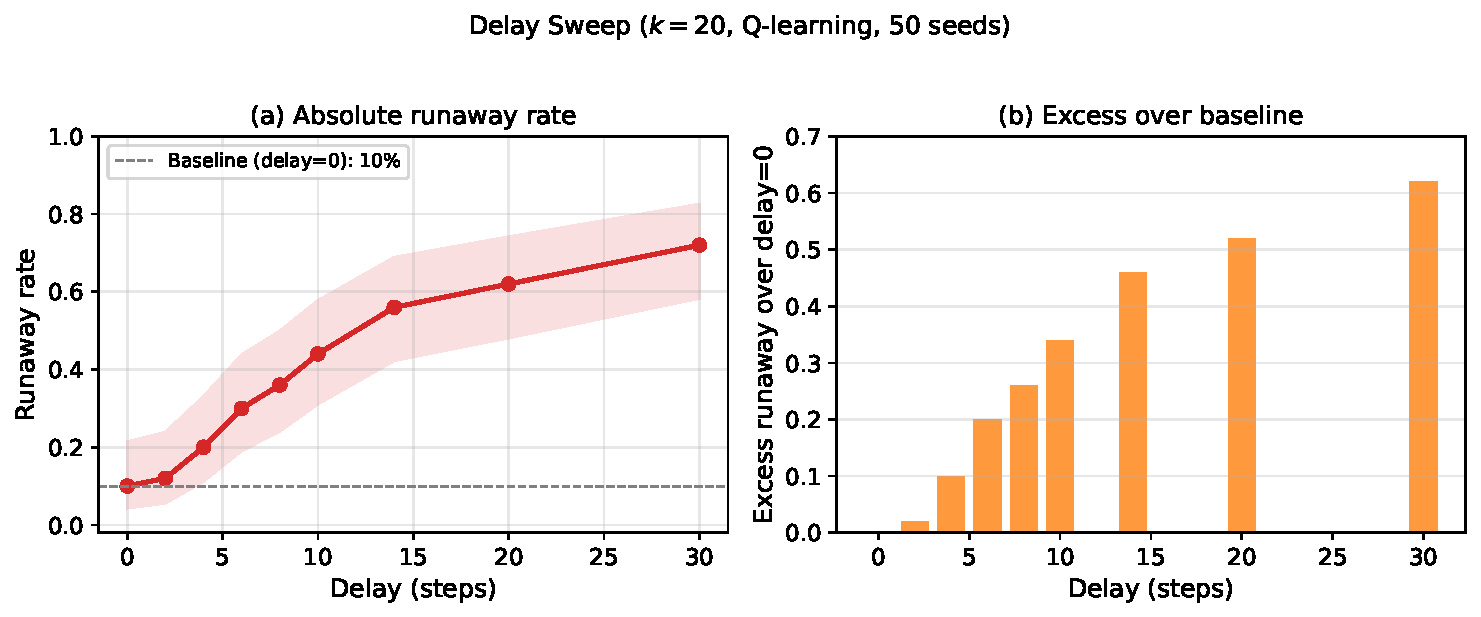
\includegraphics[width=0.85\textwidth]{figures/fig_delay_sweep.pdf}
\caption{Delay sweep (Experiment~3; $k{=}20$, Q-learning, 50 seeds). Left: runaway rate with 95\% Wilson band. Right: excess runaway over the $\Delta{=}0$ baseline. \textbf{Conclusion:} monotonic increase confirms Hypothesis~1: delay alone produces a large, dose-dependent destabilization in the networked simulation.}
\label{fig:delay_sweep}
\end{figure}

\paragraph{Experiment~4: Sharpness sweep.} This experiment tests Hypothesis~2 by holding delay fixed at 15 steps and sweeping $k \in \{3, 5, 7, 10, 15, 20, 30, 40\}$. Higher $k$ should reduce $\Delta_c$ (Equation~\ref{eq:deltac_sigmoid}), so the system should cross from stable to unstable as $k$ increases. Delay of 15 is chosen so that low-$k$ conditions are below threshold while high-$k$ conditions are above it.

At fixed delay${}{=}15$ (Table~\ref{tab:k_sweep}), runaway rate increases from 16\% ($k{=}3$) to 64\% ($k{=}40$). The transition is sharpest between $k{=}7$ (28\%) and $k{=}10$ (52\%), after which the system saturates: once operating far beyond $\Delta_c$, additional sharpening produces only marginal instability gains.

\begin{table}[ht]
\centering
\begin{tabular}{lccc}
\toprule
$k$ & Stable & Oscillatory & Runaway \\
\midrule
3  & 70\% & 14\% & 16\% \\
5  & 56\% & 24\% & 20\% \\
7  & 40\% & 32\% & 28\% \\
10 & 26\% & 22\% & 52\% \\
15 & 26\% & 14\% & 60\% \\
20 & 24\% & 16\% & 60\% \\
30 & 20\% & 18\% & 62\% \\
40 & 24\% & 12\% & 64\% \\
\bottomrule
\end{tabular}
\caption{Regime distribution by sharpness $k$ at fixed delay${}{=}15$ (Experiment~4; $N{=}240$, 500 steps, 50 seeds). \textbf{Conclusion:} runaway increases from 16\% ($k{=}3$) to 64\% ($k{=}40$), with a sharp transition at $k{=}7$--$10$ corresponding to the system crossing $\Delta_c$. This confirms Hypothesis~2 (question~2): sharpness amplifies delay vulnerability.}
\label{tab:k_sweep}
\end{table}

\begin{figure}[ht]
\centering
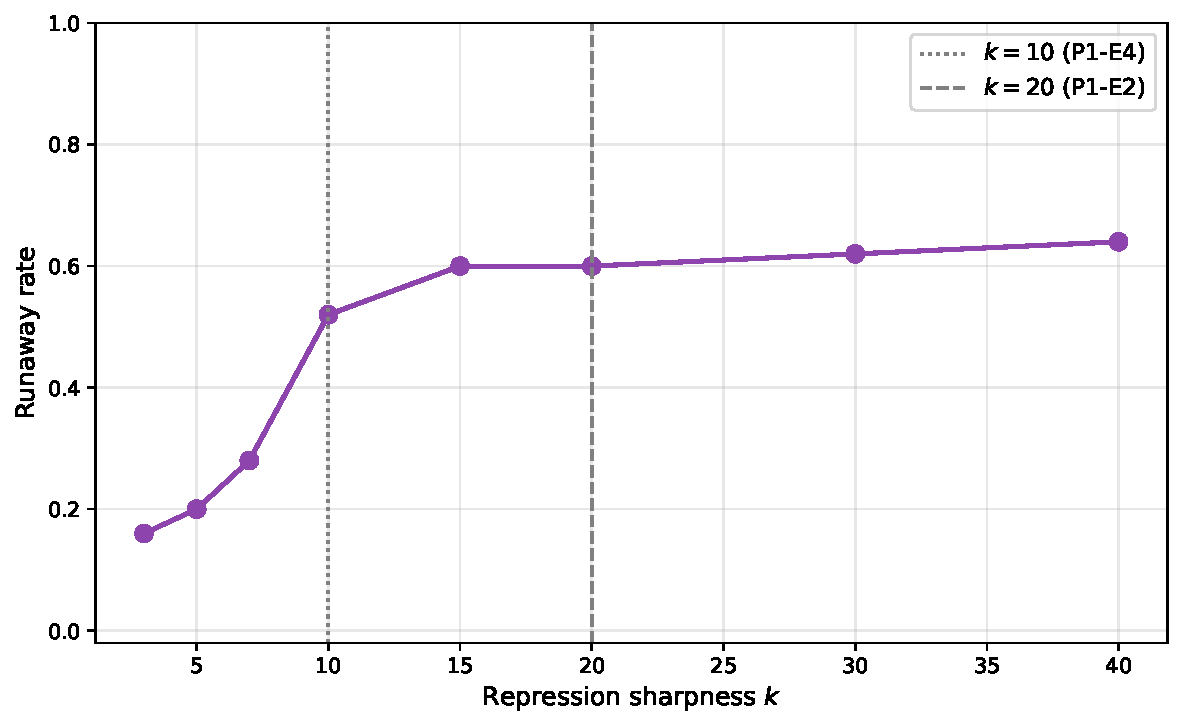
\includegraphics[width=0.75\textwidth]{figures/fig_phase_diagram.pdf}
\caption{Runaway rate vs.\ sharpness $k$ at fixed delay${}{=}15$ (Experiment~4; 50 seeds). Vertical lines: $k{=}10$ (used in Experiment~5) and $k{=}20$ (Experiment~3). \textbf{Conclusion:} the sharp transition at $k{=}7$--$10$ marks the system crossing $\Delta_c$ (Equation~\ref{eq:deltac_sigmoid}). Above this threshold, further sharpening produces diminishing returns, a ceiling effect.}
\label{fig:phase_diagram}
\end{figure}

\subsection{Central experiment: crossed delay $\times$ architecture (Experiment~5)}

This is the central experiment. A two-factor design crosses delay ($\Delta \in \{0, 4, 8, 14, 20\}$) with agent architecture: \emph{fixed-policy} (no environmental response, the null model), \emph{reactive} (threshold heuristic without memory), and \emph{Q-learning} (tabular RL with cumulative value estimates). We use $k{=}10$ to ensure fixed-policy agents remain stable as a clean baseline. The naive expectation is that learning amplifies instability; the alternative is that cumulative learning provides implicit memory that dampens oscillations.

The two-factor crossing reveals a clear hierarchy (Figure~\ref{fig:crossed} and Table~\ref{tab:crossed}).

\begin{figure}[ht]
\centering
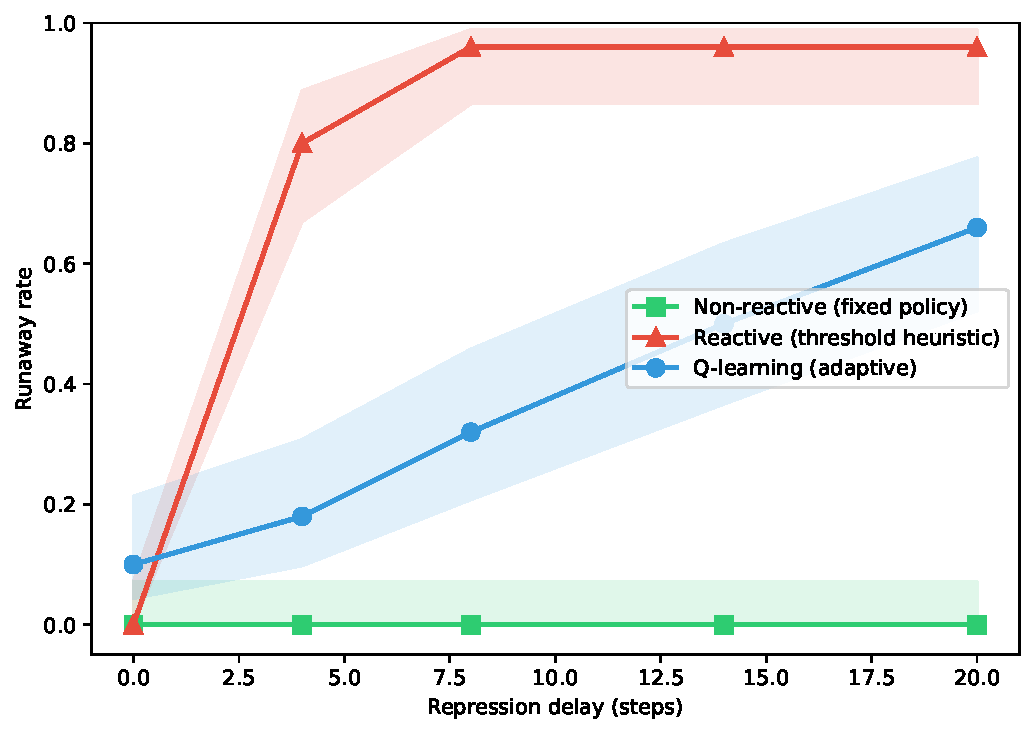
\includegraphics[width=0.75\textwidth]{figures/fig_crossed_delay_learning.pdf}
\caption{Runaway rate vs.\ delay for three agent architectures (Experiment~5, the central experiment; $k{=}10$, $N{=}240$, 500 steps, 50 seeds per cell). Shaded: 95\% Wilson CIs. \textbf{Conclusion:} the hierarchy is reactive (96\%) $>$ Q-learning (66\%) $>$ fixed (0\%). Learning \emph{buffers} rather than amplifies instability (question~3), contradicting the naive expectation. The destabilizing ingredient is memoryless reactivity to delayed signals.}
\label{fig:crossed}
\end{figure}

This experiment uses $k=10$ (lower than the aggressive $k=20$ of Experiment~3) and 500 time steps with $N=240$ agents. The results reveal three distinct regimes:

\begin{enumerate}
\item \textbf{Non-reactive (fixed):} 0\% runaway at all delays (92\% stable, 8\% oscillatory from finite-sample binomial noise in the action draws, occasionally triggering the spectral classifier). These agents cannot exploit temporal structure in the repression signal.
\item \textbf{Reactive (threshold heuristic):} fully stable without delay (100\% stable at delay${}=0$), then a sharp transition to large-amplitude runaway as delay grows: 80\% runaway at delay${}=4$, rising to 96\% at delay${}=8$ (95\% CI $[87\%, 99\%]$). A fine-resolution sweep (Figure~\ref{fig:reactive_fine}) locates the threshold sharply between delay${}=2$ (90\% stable) and delay${}=3$ (62\% runaway), the discrete-time analog of the critical delay $\Delta_c$. This is the cleanest instance of the central claim: an otherwise fully stable population destabilized by delay alone. The reactive policy immediately exploits low-alarm windows but has no memory of past punishment to dampen the resulting oscillations.
\item \textbf{Q-learning:} 10\% runaway at delay${}=0$, rising to 66\% at delay${}=20$ (95\% CI $[52\%, 78\%]$). Q-values encode cumulative punishment experience, which creates inertia against full exploitation of every low-alarm window.
\end{enumerate}

The key finding is the ordering: reactive $>$ Q-learning $>$ fixed in delay sensitivity. The immunity of fixed-policy agents is structural, not contingent on $k$: because their action distribution does not depend on the alarm signal, the feedback loop required for delay-induced instability is broken regardless of parameter values. Reactivity to delayed signals is the destabilizing mechanism; adaptive learning partially buffers this through implicit memory rather than amplifying it.

\begin{table}[ht]
\centering
\begin{tabular}{lcccc}
\toprule
Delay (steps) & Fixed & Reactive & Q-learning & 95\% CI (Q-learning) \\
\midrule
0  & 0\%  & 0\%  & 10\% & $[4\%, 21\%]$ \\
4  & 0\%  & 80\% & 18\% & $[10\%, 31\%]$ \\
8  & 0\%  & 96\% & 32\% & $[21\%, 46\%]$ \\
14 & 0\%  & 96\% & 50\% & $[37\%, 63\%]$ \\
20 & 0\%  & 96\% & 66\% & $[52\%, 78\%]$ \\
\bottomrule
\end{tabular}
\caption{Runaway rate by delay and agent architecture (Experiment~5; $k{=}10$, $N{=}240$, 500 steps, 50 seeds per cell). \textbf{Conclusion:} the ordering fixed (0\%) $<$ Q-learning (up to 66\%) $<$ reactive (up to 96\%) holds at every delay $\Delta \geq 4$; at $\Delta=0$ all three are at the floor (fixed 0\%, reactive 0\%, Q-learning 10\% from exploration noise). Q-learning's implicit punishment memory provides partial protection; memoryless reactivity is catastrophically fragile. This answers question~3: learning buffers, not amplifies, delay-induced instability.}
\label{tab:crossed}
\end{table}

\begin{figure}[ht]
\centering
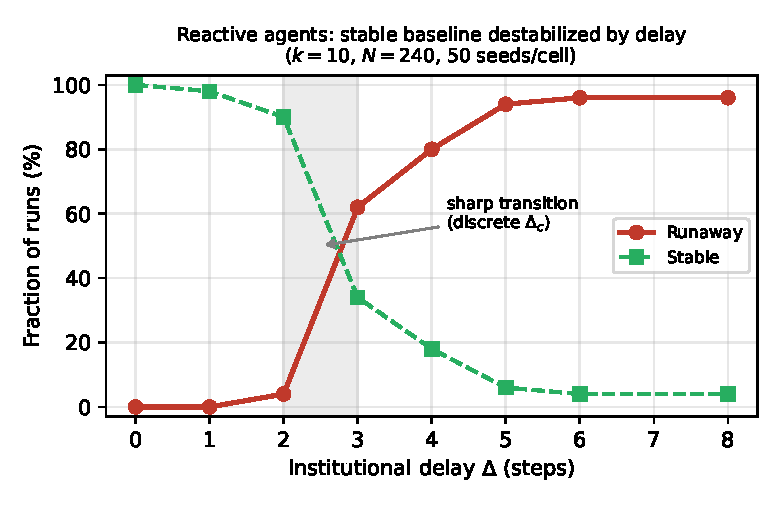
\includegraphics[width=0.6\textwidth]{figures/fig_reactive_fine.pdf}
\caption{Fine-resolution delay sweep for reactive agents ($k{=}10$, $N{=}240$, 50 seeds per delay). The population is fully stable at $\Delta=0$ and through $\Delta=2$ (90\% stable), then transitions sharply to runaway between $\Delta=2$ and $\Delta=3$---the discrete-time analog of the critical delay $\Delta_c$. \textbf{Conclusion:} delay alone, applied to an otherwise stable population, drives the destabilization (question~1).}
\label{fig:reactive_fine}
\end{figure}

\subsection{Exploratory: RL regulator (Experiment~6)}

This experiment compares three governance configurations: fixed-policy agents with a static regulator, Q-learning agents with a static regulator, and Q-learning agents with an RL-trained regulator. The RL regulator selects force $u_t \in \{0, 0.5, 1.0, 1.5, 2.0, 2.5\}$ to minimize $r_{\mathrm{reg}} = -\Rfrac - 0.1\,u_t$, where $\Rfrac$ is the radical fraction and $u_t$ is the control intensity. The regulator shares the institution's information delay, so it cannot circumvent the destabilizing lag. This experiment is exploratory: 50 seeds provide limited statistical power, and we report results as suggestive.

\begin{figure}[ht]
\centering
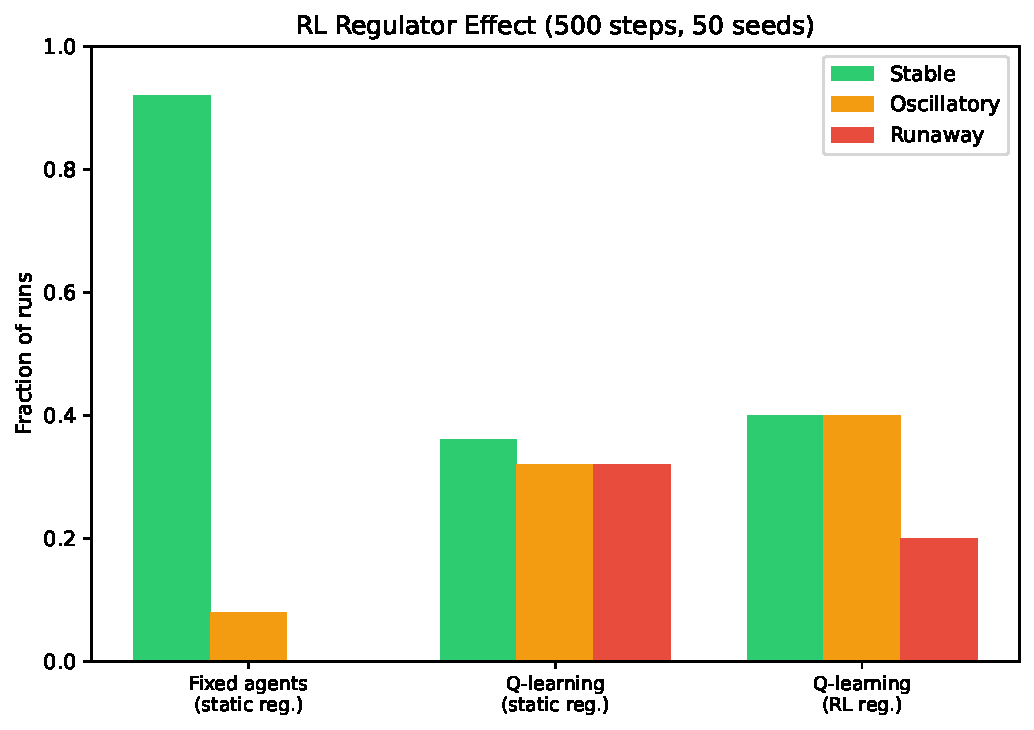
\includegraphics[width=0.65\textwidth]{figures/fig_rl_regulator.pdf}
\caption{Regime distribution for three governance configurations (Experiment~6; 500 steps, 50 seeds). \textbf{Conclusion:} the RL regulator reduces runaway from 32\% to 20\% but increases oscillations from 32\% to 40\%, suggesting mode conversion (disaster into bounded oscillation) rather than full stabilization. The effect is suggestive but not statistically conclusive at 50 seeds (question~4).}
\label{fig:rl_regulator}
\end{figure}

The learning ablation compares three governance configurations (Table~\ref{tab:ablation}). Fixed-policy agents achieve 92\% stability, establishing the baseline. Q-learning agents with a static regulator produce 36\% stable, 32\% oscillatory, and 32\% runaway. Introducing an RL-trained regulator (a Q-learning agent that observes the delayed alarm and radical fraction, selects force $u_t \in \{0, 0.5, 1.0, 1.5, 2.0, 2.5\}$, and receives reward $r_{\mathrm{reg}} = -\Rfrac - 0.1\,u_t$, where $\Rfrac$ is the radical fraction) shifts the distribution to 40\% stable, 40\% oscillatory, and 20\% runaway. This result is suggestive rather than conclusive: the 12 percentage-point reduction in runaway (32\% to 20\%) on 50 seeds yields a confidence interval that includes zero effect. The simultaneous increase in oscillatory outcomes from 32\% to 40\% suggests that if the regulator does help, it converts catastrophic runaway into bounded oscillations rather than restoring stability. We treat this as exploratory evidence that adaptive governance can transform instability modes, not as a confirmed finding.

\begin{table}[ht]
\centering
\begin{tabular}{lccc}
\toprule
Condition & Stable & Oscillatory & Runaway \\
\midrule
Fixed agents (static regulator) & 92\% & 8\% & 0\% \\
Q-learning (static regulator)   & 36\% & 32\% & 32\% \\
Q-learning (RL regulator)       & 40\% & 40\% & 20\% \\
\bottomrule
\end{tabular}
\caption{Regime distribution by governance configuration (Experiment~6; 50 seeds each). \textbf{Conclusion:} adaptive governance converts runaway into oscillation (32\%$\to$20\% runaway, 32\%$\to$40\% oscillatory) rather than restoring stability. This mode conversion is the realistic ceiling for a controller sharing the institution's delay (question~4, exploratory).}
\label{tab:ablation}
\end{table}

\subsection{Summary of findings}

The central result is the two-factor crossing (Experiment~5): reactive agents collapse catastrophically under delay (96\%), Q-learning agents achieve partial resilience (66\%), and non-reactive agents are immune (0\%). Reactivity is the destabilizing mechanism; learning buffers it. The story is simpler than one might expect. The ODE validation (Experiment~1) and discrete mean-field (Experiment~2) confirm that the analytical mechanism is correct and survives discretization. The delay sweep (Experiment~3) and sharpness sweep (Experiment~4) map the dose-response and activation boundary. The RL regulator (Experiment~6) is exploratory: suggestive of mode conversion but not statistically conclusive.

All regime classifications use the adaptive classifier with runaway threshold $R_{\max}>0.40$. The quantitative gap between mean-field thresholds and simulation thresholds reflects the expected difference between an analytically tractable mechanism and a system with agent heterogeneity, stochastic exploration, and network structure.
